\scanpage{114}
\margin{\figure{\begin{tikzpicture}\draw[brown!65!black,line width=.45pt] (0,0) .. controls (.01,-.25) and (.035,-.65) .. (.02,-.8);\end{tikzpicture}}}
est de plus propre, alors pour \uline{toute} sous-variété linéaire $\inserted{L_t}$ de codimensio\handwritten{n} $s$, $Y_t=f_t^{-1}(L_t)$ est géométriquement connexe.

Conjuguant avec 2, on trouve, par l'argument qui a permis de déduire 3 de 1 :

\margin{\handwritten{\shortstack[l]{cf.\\\unsure{SCA|SGA} 1 X $2\unsure{,|.}\unsure{11|II}$}}}
\margin{\figure{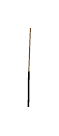
\begin{tikzpicture}\draw[brown!55!black,line width=.35pt] (.025,0)--(.005,-.55);\draw[black,line width=.55pt] (.005,-.55)--(0,-1);\end{tikzpicture}}}
\uline{Corollaire} 5: \deleted{Avec}\inserted{\handwritten{Sous}} les hypothèses de \unsure{3|4} , \inserted{avec $X$ propre,} l'homomorphisme danonique $\handwritten{\pi}_1(Y_{\bar t})\handwritten{\rightarrow}\handwritten{\pi}_1(X)$ ($\handwritten{\simeq}\handwritten{\pi}_1(X_{\bar t})$ par le théorème de changement de base) est surjectif.

Nous désirons également un énoncé analogue à 5, donnant une surjectivité pour des $\handwritten{\pi}_1$ pour un $t$ non générique, mais sans hypothèse de propreté, et pour des quotients plus gros du $\handwritten{\pi}_1$ que ceux envisagés dans (**). On peut\deleted{nt} donner à ce sujet le résultat suivant:

\margin{\figure{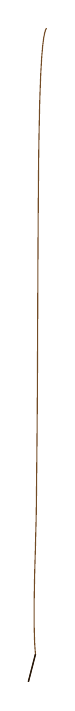
\begin{tikzpicture}\draw[brown!60!black,line width=.4pt] (.15,0) .. controls (.01,-.18) and (.06,-3.1) .. (.02,-6.15) .. controls (.01,-6.75) and (-.03,-7.5) .. (.01,-7.95) --(-.08,-8.3);\draw[black!80!brown,line width=.5pt] (.01,-7.95)--(-.08,-8.3);\end{tikzpicture}}}
\uline{Théorème} 6. Su\unsure{p|i}\unsure{p|t}osons $k$ algébriquement clos, \inserted{\handwritten{et}} $X$ propre, $f:X\handwritten{\rightarrow}P^r$, \deleted{et} le sous -espace linéaire $L_t$ de $P^r$ de codimension $s$ (défini sur $k$, pour fixer les idées) \deleted{tels qu'on ait} et enfin le sous-schéma fermé $D$ de $X$ tels qu'on ait ceci; \deleted{où on a posé $U=X-D$}

a) \deleted{$U_t=U\unsure{\cap}X_t$ et} $\deleted{X}\handwritten{Y}_t=f^{-1}(L_t)$ est non vide.

b) Pour tout $x\handwritten{\in}\deleted{X}\handwritten{Y}_t$ , $X$ est lisse en $x$, $Y_t$ est lisse en $x$\handwritten{,} de codi\unsure{memt|ment}sion $s$ dans $X$ en $x$, $f$ est net en $x$.

c) Pour tout $x\handwritten{\in}D_t=D\handwritten{\cap}Y_t$ , o\deleted{\`{}}u \deleted{bien} bien $\operatorname{codim}_x(D_t,\mathord{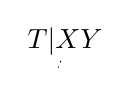
\begin{tikzpicture}[baseline=(g.base),x=1em,y=1em]\node[inner sep=0pt] (g) at (0,0) {$\deleted{\unsure{T|X}}\handwritten{Y}$};\fill[black] (-.17,-.73) ellipse (.026 and .036);\fill[brown!60!black] (-.24,-.92) circle (.03);\end{tikzpicture}}_t)\handwritten{\geqslant}2$, ou bien $D_{\deleted{\unsure{t}}}$ est un diviseur \unsure{e|s}\unsure{u|n}r $X$ en $x$ et $\deleted{D_t}$ induit sur $Y_t$ en $x$ un diviseur à croisements normaux.

Supposons $U=X-D$ irréductible, et considérons l'inclusion $U_t=U\handwritten{\cap}Y_t\handwritten{\longrightarrow}U$ . \deleted{Alors $U_t$} Soit $\handwritten{\pi}_1^t(U)$ le \deleted{grou} quotient du groupe fondamental de $U$ \deleted{formé des} qui classifie les revêtements de $U$ qui sont modérément ramifiés en les composantes irréductibles de codimension 1 de $D$ dans $X$ qui rencontrent $Y_t$, \deleted{(\unsure{i.e.} telles que $D$} et $\overset{\unsure{\scriptscriptstyle t|+}}{\handwritten{\pi}}_1^t(\unsure{U|V}_t)$ le quotient \deleted{analogue} de $\handwritten{\pi}_1(U_t)$ qui classifie les revêtements qui sont modérément ramifiés en les composantes irréductibles de codimension 1 de $D_t$ . On a un homomor%
% The last visible fragment ends in a line-ending hyphen in the image; suppressed under the joining convention, with no continuation supplied.
% archive sheet number: 113
